\chapter{Megvalósítás}
\label{ch:implementation}

A fejezet a terv megvalósításának azokat a részeit mutatja be, ahol a megoldás nem magától értetődő. Ilyen a találatvizsgálat, az elforgatott alakzatok méretezése, a körívek és a szabadkézi vonalak előállítása, a logikai műveletek, a szöveg útvonallá alakítása, az SVG importálása és az érintéses használat. A programkódok rövidített részletek, a megjegyzéseik a forráskódhoz igazodva angol nyelvűek.

\section{A fejlesztés menete}
\label{sec:dev_process}

A szerkesztő több fejlesztési körben, fokozatosan készült. Egy kör egy funkciócsoport megvalósításával kezdődött, például a logikai műveletekkel, a betűtípusok kezelésével vagy az érintéses vezérléssel, és az új kódhoz automatikus tesztek is készültek. Ezután a felületet böngészőben végigpróbáltam, a talált hibákat és a használat közben felmerült módosítási igényeket listába gyűjtöttem, és ezek adták a következő kör feladatait. A kézi tesztelésből származó hibák regressziós tesztjeit \aref{sec:manual_tests}. szakasz mutatja be.

A szerkesztő \aref{tab:versions}. táblázatban felsorolt könyvtárakra és a vele szállított, SIL Open Font License alatt terjesztett betűtípusokra épül. Minden más, így az adatmodell, az előzménykezelés, az eszközök, a geometriai számítások nagy része, az SVG-importáló és -exportáló, a betűtípusok kezelése, a felület komponensei és a tesztek a projekt keretében készültek.

A tervezési döntéseket és azok indoklását a forráskód mellett egy döntési napló, az alkalmazás felépítését egy architektúra-leírás rögzíti, mindkettő megtalálható a mellékelt adathordozón. A munka a dolgozat alapján megismételhető. A függőségek pontos verzióit \aref{tab:versions}. táblázat tartalmazza, a telepítés, a futtatás és a tesztek indításának lépéseit pedig az adathordozó leírása sorolja fel.

\section{A projekt felépítése}
\label{sec:project_structure}

A forráskód az \texttt{src} mappában van. A belépési pont a \texttt{main.ts}, amely az \texttt{App.svelte} gyökérkomponenst jeleníti meg az oldalon, a többi kód pedig az \texttt{src/lib} almappáiban található, \aref{sec:architecture}. szakaszban leírt rétegek szerint. A mappák tartalmát és méretét \aref{tab:source-size}. táblázat foglalja össze.

\begin{table}[!htbp]
\caption{A forráskód mappái}
\label{tab:source-size}
\centering
\footnotesize
\begin{tabular}{|l|>{\raggedright\arraybackslash}p{0.55\textwidth}|r|r|}
\hline
\textbf{Mappa} & \textbf{Tartalom} & \textbf{Fájl} & \textbf{Sor} \\ \hline
\texttt{utils} & adatmodell, geometria, útvonalak, SVG-import és -export, logikai műveletek, vágólap & 32 & 5183 \\ \hline
\texttt{stores} & dokumentum és előzmények, felület, nézet, szerkesztési műveletek & 11 & 1158 \\ \hline
\texttt{tools} & a tizenhárom eszköz és közös segédfüggvényeik & 18 & 1270 \\ \hline
\texttt{fonts} & betűtípus-katalógus, Google Fonts, helyi és beépített betűtípusok & 17 & 1429 \\ \hline
\texttt{components} & újrahasználható komponensek, például a színválasztó, az objektumlista és a párbeszédablakok & 20 & 2850 \\ \hline
\texttt{layouts} & a felület nagy egységei: vászon, menü, parancssáv, panelek & 6 & 2060 \\ \hline
\end{tabular}
\end{table}

A gyökérkomponenssel és a globális stíluslappal együtt a forráskód körülbelül 14\,300 sor. A tesztek a \texttt{tests} mappában vannak, ezeket \aref{ch:test}. fejezet mutatja be.

\section{Megjelenítés és találatvizsgálat}
\label{sec:rendering}

A vászon maga is egy SVG-elem, amelyben a \texttt{ShapeRenderer} komponens rajzolja ki az alakzatokat. A komponens ugyanazokat az attribútumokat írja ki, mint az exportáló, így a képernyőn látott kép megegyezik a mentett fájllal. Az értékeket mindig kiírja, akkor is, ha megegyeznek az SVG alapértékeivel, mert a szerkesztő alapértékei eltérnek azoktól. Az SVG alapértelmezett vonalvége például a levágott \texttt{butt}, a sarka a hegyes \texttt{miter}~\cite{w3c-svg-painting}, a szerkesztőben viszont mindkettő lekerekített.

Minden kattintásnál el kell dönteni, mi van a mutató alatt: egy alakzat, egy fogantyú, egy csomópont vagy az üres vászon. Ezt a feladatot találatvizsgálatnak, angolul \textit{hit-testing}nek nevezik. Elforgatott alakzatokra, vastag körvonalakra, görbékre és szövegekre pontosan kiszámolni sok geometriai kódot igényelne. A böngésző viszont ezt a számítást már elvégzi, mégpedig pontosan úgy, ahogyan az elemeket kirajzolja, és a szerkesztő rá bízza a feladatot. Minden kirajzolt elem egy \texttt{data-} kezdetű attribútummal jelzi, mit ábrázol, egy alakzat például \texttt{data-shape-id}, egy méretező fogantyú \texttt{data-handle} attribútummal. Az esemény célelemétől a szülők felé haladva az első ilyen attribútum megmondja, mire kattintott a felhasználó.

Két esetben a böngésző viselkedését ki kellett egészíteni. Egy vékony vonalat vagy egy kitöltés nélküli útvonalat nehéz eltalálni, mert csak a körvonala kattintható. Az ilyen alakzatok alá a szerkesztő egy láthatatlan másolatot rajzol, amelynek körvonala a képernyőn legalább tíz képpont széles, és a CSS \texttt{pointer-events} tulajdonsága szerint csak ez a körvonal fogadja a mutató eseményeit~\cite{mdn-pointer-events-css}. A zárolt alakzatok \texttt{pointer-events: none} beállítást kapnak, és a kattintások átmennek rajtuk az alattuk lévő elemekre. Egy zárolt háttér így sem kijelöléssel, sem területkijelöléssel, sem vágással, sem a foltecsettel nem módosulhat véletlenül.

\section{Nézet, nagyítás és illesztés}
\label{sec:viewport}

A rajzterületnek nincsenek görgetősávjai és szélei. A nézetet egy eltolás és egy nagyítási arány írja le, az eltolás pedig a tervezőprogramokhoz hasonlóan tetszőleges lehet. Görgetősávokkal a nézet csak a lap és egy margó területén mozoghatna, a szerkesztő viszont a lapon kívüli alakzatokat is megengedi. A nagyítás 5\% és 2000\% között állítható.

Nagyításkor a kurzor alatti dokumentumpontnak a helyén kell maradnia. Legyen $s$ a nézet eltolása, $a$ a kurzor távolsága a rajzterület szélétől, $p$ a lap előtti állandó margó, $z_0$ a régi és $z_1$ az új nagyítás. A kurzor alatti dokumentumkoordináta $(s+a-p)/z_0$, és ennek az új nagyítás mellett is $a$ távolságra kell lennie. Ebből az új eltolás:
\[
s' = \frac{s + a - p}{z_0}\, z_1 + p - a .
\]
Ugyanezt a képletet használja a görgő, a két ujjas nagyítás és a nagyító gombok is, az utóbbiak a rajzterület középpontjával.

Az illesztés a mozgatott vagy rajzolt alakzat széleit és középvonalait veti össze a többi alakzat, a lap és a segédvonalak megfelelő koordinátáival. Egy koordináta akkor illeszkedik, ha legfeljebb hat képernyőpontnyira van a céltól. A küszöb a képernyőn állandó, dokumentumegységben a nagyítással osztva kell számolni. Az illesztést jelző vonalak vékony világos szegélyen futnak, így egy rózsaszín jelzővonal egy rózsaszín alakzaton is látható marad.

\section{Az előzmények megvalósítása}
\label{sec:history_impl}

\Aref{sec:history_design}. szakaszban leírt idővonalat a \texttt{documentStore} valósítja meg. Központi függvénye a \texttt{commit}, amelyet \aref{lst:commit}. programkód mutat. A függvény egy átalakítást kap, amely a régi dokumentumból újat készít. Ha az átalakítás ugyanazt az objektumot adja vissza, a művelet semmit sem változtatott, és nem keletkezik bejegyzés. Ha a hívás összevonási kulcsot is megad, és az előző lépés egy másodpercen belül ugyanezzel a kulccsal történt, az új állapot a legutóbbi bejegyzés helyére kerül.

\begin{lstlisting}[style=TS, caption={Egy visszavonható lépés rögzítése (\texttt{stores/document.ts}, rövidítve)}, label=lst:commit]
commit(label: string, fn: (d: DocumentState) => DocumentState,
       opts?: { coalesce?: string }) {
  core.update(c0 => {
    const c = cancelled(c0);              // drop an unfinished preview
    const next = fn(c.present.doc);
    if (next === c.present.doc) return c; // nothing changed: no entry
    const now = Date.now(), key = opts?.coalesce ?? null;
    if (key && key === c.lastKey && now - c.lastTime < COALESCE_MS)
      return { ...c, present: { doc: next, label: c.present.label },
               future: [], lastTime: now };          // merge
    return { past: trim([...c.past, c.present]),     // at most 200
             present: { doc: next, label }, future: [],
             base: null, lastKey: key, lastTime: now };
  });
}
\end{lstlisting}

A vásznon történő húzáshoz a tároló előnézeti módot kínál. A \texttt{beginPreview} megjegyzi a húzás előtti állapotot, ezután a \texttt{preview} hívások bejegyzés nélkül módosítják a jelenlegi állapotot, a \texttt{commitPreview} pedig egyetlen lépésként rögzíti a húzás eredményét. A \texttt{cancelPreview} visszaállítja a megjegyzett állapotot, ezt hívja például az Esc billentyű húzás közben. Az előzmények panelen egy bejegyzésre kattintva a \texttt{goTo} függvény az idővonalat a kiválasztott pontnál osztja ketté, és onnan a visszavonás és a megismétlés ugyanúgy folytatható.

Mivel a modell függvényei a változatlan részekre a régi hivatkozást tartják meg, két dokumentumállapot összehasonlítása egyetlen hivatkozás-összehasonlítás. Erre épül a fenti üres műveletek kiszűrése, és ugyanígy dönti el a szerkesztő azt is, hogy van-e mentetlen változás.

\section{Rajzoló eszközök}
\label{sec:drawing_tools}

A rajzoló eszközök közül a téglalap, az ellipszis, a vonal és a sokszög egyszerű húzásokból és kattintásokból állítja elő az alakzatot. A toll, a körív és a szabadkézi rajz megvalósítása több számítást igényel, ezért ez a szakasz ezekkel foglalkozik.

\subsection{Toll és körív}

A toll a tervezőprogramokban megszokott módon működik. Egy kattintás sarokpontot helyez el, egy húzás sima csomópontot, amelynek fogantyúit a húzás iránya és hossza adja meg. Az útvonalat dupla kattintás, az Enter vagy az Esc billentyű fejezi be, az első pontra kattintás pedig bezárja.

A körív eszköz három ponttal dolgozik, a két végponttal és egy harmadikkal, amelyen az ívnek át kell haladnia. Ez a mozdulat egérrel és ujjal is ugyanúgy végrehajtható. A három pont meghatározza a köréjük írható kört. Ha a pontokat a harmadik ponthoz, $P$-hez viszonyítva $\mathbf{a} = A - P$ és $\mathbf{b} = B - P$ jelöli, a kör középpontja
\[
C = P + \frac{1}{d}\Bigl(b_y |\mathbf{a}|^2 - a_y |\mathbf{b}|^2,\; a_x |\mathbf{b}|^2 - b_x |\mathbf{a}|^2\Bigr),
\qquad d = 2\,(a_x b_y - a_y b_x).
\]
Ha $d$ közel nulla, a három pont egy egyenesre esik, és az eszköz egyenes szakaszt rajzol. A Shift billentyű lenyomásakor az ív középponti szöge tizenöt fokos lépésekben változik, így negyed- és félkör is pontosan beállítható.

A modell csak harmadfokú Bézier-görbéket ismer, ezért a körívet közelíteni kell. Egy $\varphi$ középponti szögű, $r$ sugarú ív egyetlen harmadfokú görbével akkor közelíthető jól, ha a két fogantyú az ív érintőjének irányába mutat, és a hosszuk
\[
h = \frac{4}{3}\tan\frac{\varphi}{4}\; r .
\]
Negyedkörre ez a sugár körülbelül 0{,}5523-szorosa, a közelítés legnagyobb eltérése pedig a sugár 0{,}027\%-a~\cite{goldapp1991,bezier-primer}. Nagyobb szögeknél a hiba gyorsan nő, ezért az eszköz az ívet legfeljebb 90 fokos darabokra bontja, ahogyan \aref{lst:arcnodes}. programkód mutatja.

\begin{lstlisting}[style=TS, caption={Körív felbontása Bézier-csomópontokra (\texttt{utils/arc.ts}, rövidítve)}, label=lst:arcnodes]
export function arcNodes(arc: Arc): PathNode[] {
  const k = Math.max(1, Math.ceil(Math.abs(arc.sweep) / (Math.PI / 2) - 1e-9));
  const phi = arc.sweep / k;                        // at most 90 degrees
  const h = (4 / 3) * Math.tan(phi / 4) * arc.r;    // handle length
  const nodes: PathNode[] = [];
  for (let i = 0; i <= k; i++) {
    const ang = arc.start + phi * i, p = at(ang), tg = tangent(ang);
    nodes.push({ x: p.x, y: p.y,
      hin:  i > 0 ? { x: p.x - tg.x * h, y: p.y - tg.y * h } : null,
      hout: i < k ? { x: p.x + tg.x * h, y: p.y + tg.y * h } : null,
      smooth: i > 0 && i < k });
  }
  return nodes;
}
\end{lstlisting}

A toll és a körív egy közös, éppen rajzolt útvonalon dolgozik, amelyet a \texttt{pathDraft} modul tárol. Minden új ív ott kezdődik, ahol az előző szakasz véget ért, így a körív eszköz a tollhoz hasonlóan használható. A szakaszok egymást követik, a rajzolást dupla kattintás vagy az Enter billentyű zárja le. Ha a rajzolás egy kijelölt nyitott útvonal végpontján kezdődik, a közös vázlat ezt az útvonalat veszi át. Az új szakaszok hozzá kerülnek, az alakzat megtartja azonosítóját, nevét és stílusát, a másik végpontjára kattintva pedig bezárul. Ugyanezt a végpontkeresést használja a szabadkézi eszköz is.

\subsection{Szabadkézi rajz}

Az egér vagy az ujj mozgása sok mintát ad, amelyekből közvetlenül egy töröttvonal is készülhetne. Ez azonban sok száz csomópontot jelentene, és a kéz remegését is megőrizné, ezért az eszköz két lépésben dolgozza fel a mintákat.

Az első lépés a Ramer-Douglas-Peucker algoritmus~\cite{ramer,douglas-peucker}. Az algoritmus a két végpontot összekötő szakasztól legtávolabbi mintát keresi. Ha ez a távolság egy tűréshatárnál nagyobb, a pontot megtartja, és a két keletkező részre megismétli a keresést, különben a köztes pontokat elhagyja. A megvalósítás rekurzió helyett saját vermet használ, hogy egy hosszú vonal se tölthesse meg a hívási vermet. A tűréshatár a képernyőn nagyjából másfél képpont, így erősebb nagyításnál a vonal részletesebb marad.

A második lépés a megmaradt pontokból sima görbét készít. A $P_i$ csomópont fogantyúi a szomszédos pontokat összekötő irányba mutatnak, a Catmull-Rom spline-ok mintájára~\cite{catmull1974}:
\[
\mathbf{t}_i = \frac{P_{i+1} - P_{i-1}}{6}, \qquad
H^{\mathrm{be}}_i = P_i - \mathbf{t}_i, \qquad H^{\mathrm{ki}}_i = P_i + \mathbf{t}_i .
\]
Az eredmény néhány tucat sima csomópont, amely a csomóponteszközzel kényelmesen tovább alakítható.

\section{Alakzatok szerkesztése}
\label{sec:editing}

A már megrajzolt alakzatokat a kijelölő eszköz mozgatja, méretezi és forgatja, a csomóponteszköz pedig az alakjukat módosítja. Mindkettőnél az okozza a nehézséget, hogy az alakzatok el lehetnek forgatva.

\subsection{Elforgatott alakzatok méretezése}

Egy elforgatott alakzat méretezésekor a megfogott fogantyúval szemközti saroknak vagy élnek a helyén kell maradnia. Az alakzat forgatása a határoló téglalap közepe körül értendő, a méretezés viszont elmozdítja ezt a középpontot, és egy egyszerű méretezés után az alakzat elcsúszna. A \texttt{resizeShape} függvény ezért három lépésben dolgozik.

\begin{enumerate}
\item A mutató helyét a forgatás középpontja körül $-\theta$ szöggel visszaforgatja, így a mutató az alakzat saját, el nem forgatott koordináta-rendszerébe kerül.
\item Ebben a rendszerben a megfogott fogantyú szerint új határoló téglalapot számol, Shift billentyűvel az arányokat megtartva, és az alakzatot ebbe a téglalapba méretezi.
\item A rögzített pont helyét a régi és az új téglalapban is kiszámolja, mindkettőt a saját középpontja körül $\theta$ szöggel elforgatva. A két pont különbségével eltolja az alakzatot, és a rögzített pont a képernyőn ugyanott marad.
\end{enumerate}

Több kijelölt alakzat a közös, tengelyekkel párhuzamos határoló téglalap szerint méreteződik. Minden alakzat középpontja a téglalappal együtt mozog, a mérete ugyanolyan arányban változik, a forgatása pedig megmarad. Ez eltolásra és arányos méretezésre pontos, egy elforgatott alakzat nem arányos méretezése viszont csak közelítés, mert a modell nem ismeri a nyírást. Ugyanez a szabály érvényes a csoportok tagjaira is.

\subsection{A forgatási középpont}

\Aref{sec:data_model}. szakasz szerint az áthelyezett forgatási középpont csak a forgatás végrehajtását befolyásolja. Ha egy alakzatot $\Delta$ szöggel egy tetszőleges $O$ pont körül kell elforgatni, a szerkesztő a tárolt szöghöz hozzáadja $\Delta$-t, a téglalap $C$ középpontját az $O$ pont körül elforgatja, és az alakzatot az új középpontba tolja. Az eredmény ugyanaz, mintha az alakzat valóban az $O$ pont körül fordult volna el, az exportált fájlban azonban továbbra is egyetlen \texttt{rotate} transzformáció szerepel. A geometria panel is ezt a műveletet végzi, amikor a felhasználó számmal adja meg a szöget.

\subsection{Csomópontok szerkesztése}

A csomóponteszköz, a felületen \textit{Edit Nodes}, minden alakzattípushoz szerkeszthető pontokat kínál. Útvonalnál ezek a csomópontok és a fogantyúk, téglalapnál a saroksugarak, ellipszisnél a két sugár, vonalnál a végpontok. A pontok az alakzat saját, el nem forgatott koordináta-rendszerében értendők, és ugyanaz a kód kezeli az elforgatott és a nem elforgatott alakzatokat.

Több csomópont is kijelölhető Shift-kattintással vagy egy téglalap húzásával, akár az alakzat belsejéből indítva. A kijelölt csomópontok együtt mozognak, a nyílbillentyűkkel léptethetők, együtt törölhetők, és mindegyik fogantyúja látszik. Dupla kattintás az útvonalon új csomópontot illeszt be, egy csomóponton pedig a sarok és a sima típus között vált. \Aref{fig:edit-nodes}. ábra egy kulcslyuk alakú útvonalat mutat két kijelölt csomóponttal.

\begin{figure}[!htbp]
\centering
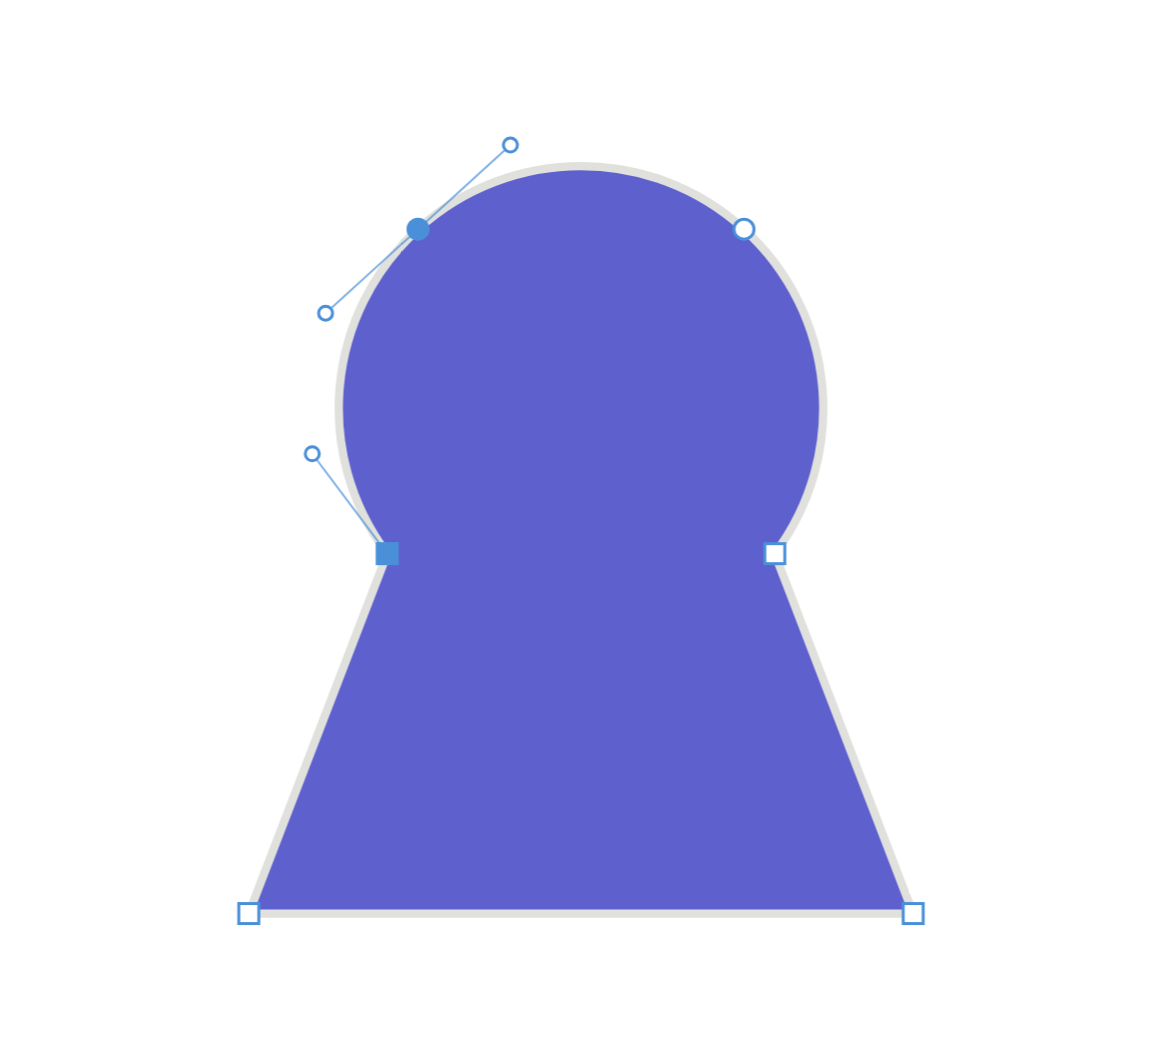
\includegraphics[width=0.5\textwidth]{images/editor/edit-nodes.png}
\caption{Két kijelölt csomópont a fogantyúival}
\label{fig:edit-nodes}
\end{figure}

A fogantyúk abszolút koordinátákként tárolódnak, nem a csomóponthoz viszonyított eltolásként. Az eltolás, a méretezés és a tükrözés emiatt minden pontra ugyanaz a leképezés, a csomópontokat és a fogantyúkat nem kell külön kezelni. Sima csomópontnál az egyik fogantyú mozgatása a másikat az ellenkező irányba igazítja, és a görbe törés nélkül halad át a csomóponton.

\section{Logikai műveletek és vágás}
\label{sec:boolean_impl}

A logikai műveletek a paper.js könyvtár \texttt{unite}, \texttt{subtract}, \texttt{intersect} és \texttt{exclude} metódusaira épülnek~\cite{paperjs}. A szerkesztő a kijelölt alakzatokat előbb paper.js útvonalakká alakítja. A téglalapok, ellipszisek és vonalak ehhez útvonallá válnak, a forgatás beépül a csomópontok koordinátáiba, a fogantyúk pedig a csomóponthoz viszonyított értékekre alakulnak, mert a paper.js ezt a formát várja. Az eredményt ugyanígy alakítja vissza.

A műveletek a halmozási sorrendet követik. Az unió, a metszet és a kizárás eredménye a legfelső alakzat stílusát kapja. A különbség a legalsó alakzatból vágja ki az összes többit, és a legalsó stílusát tartja meg. A felosztás minden alakzatot a körvonalaik által kijelölt darabokra bontja, és minden darab annak az alakzatnak a stílusát kapja, amelyik legfelül fedi. A paper.js dokumentációja szerint a felosztás egy különbség és egy metszet együttese~\cite{paperjs}. Több alakzatra a szerkesztő ezt lépésenként terjeszti ki. Minden következő alakzat az eddigi darabokat egy rajta kívüli és egy vele közös részre vágja, saját magából pedig az eddig le nem fedett rész lesz új darab. A felületen a műveletek \textit{Unite}, \textit{Subtract}, \textit{Intersect}, \textit{Exclude} és \textit{Divide} néven érhetők el. \Aref{fig:boolean}. ábra két egymást fedő alakzaton mutatja az öt műveletet.

\begin{figure}[!htbp]
\centering
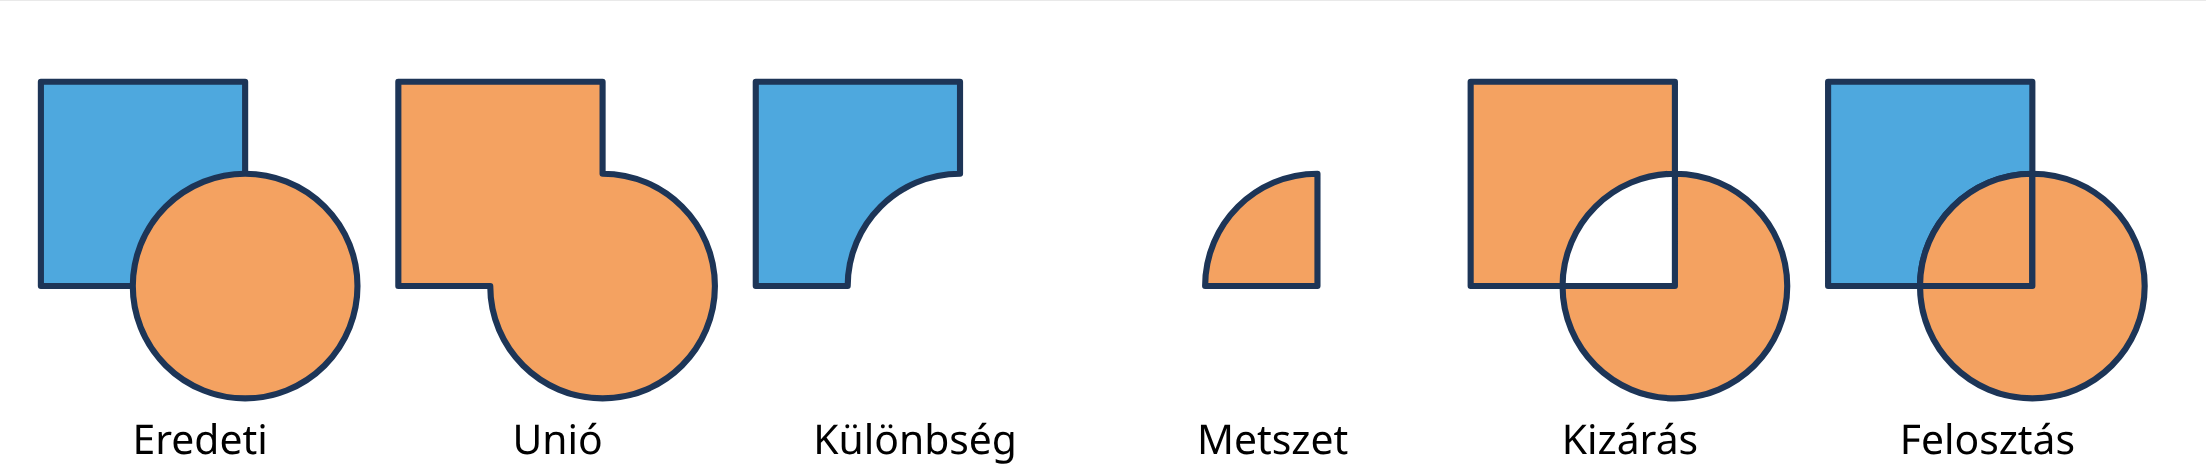
\includegraphics[width=\textwidth]{images/editor/boolean.png}
\caption{Két alakzat és a rajtuk végzett öt logikai művelet eredménye}
\label{fig:boolean}
\end{figure}

Az olló eszköz kétféleképpen vág. Egy kattintás az útvonal körvonalán csak abban a pontban vágja el az útvonalat: egy nyitott útvonal két részre esik, egy zárt útvonal pedig ott kinyílik. A vágás helyére új csomópont kerül, amelyet a de Casteljau-algoritmus számol ki~\cite{farin2002}, így az alakzat alakja nem változik. Egy húzás ezzel szemben kést rajzol, amely mentén minden eltalált alakzat kettéválik. Zárt alakzatnál a darabok is zártak, vagyis a körvonal a vágás mentén is végigfut.

Egy vonalnak nincs területe, ezért közvetlenül nem lehet logikai művelet operandusa. A szerkesztő a késből egy területet épít, ahogyan \aref{lst:knife}. programkód mutatja. A kés két végét az érintő irányában messzire meghosszabbítja, és a vonalat az egyik oldalán körbezárja. A darabok ezután egy metszet és egy különbség eredményeként állnak elő. Ha a felhasználó a kést a kiindulópontjáig visszahúzza, az lasszóként működik, és maga a zárt vonal lesz a vágó terület.

\begin{lstlisting}[style=TS, caption={A késből épített vágó terület (\texttt{utils/boolean.ts})}, label=lst:knife]
export function knifeRegion(paper: Paper, knife: Item, far: number): Item {
  const first = knife.firstSegment.point, last = knife.lastSegment.point;
  const t0 = knife.getTangentAt(0).normalize();
  const t1 = knife.getTangentAt(knife.length).normalize();
  const start = first.subtract(t0.multiply(far)), end = last.add(t1.multiply(far));
  const dir = end.subtract(start).normalize();
  const side = new paper.Point(-dir.y, dir.x).multiply(far * 2);
  const region = knife.clone({ insert: false });
  region.insert(0, start);
  region.add(end, end.add(side), start.add(side));
  region.closed = true;
  return region;
}
// the two pieces:  target.intersect(region)  and  target.subtract(region)
\end{lstlisting}

\section{Körvonalak}
\label{sec:strokes}

A körvonal beállításai közül a szaggatás és a körvonal útvonallá alakítása igényelt saját megoldást. Ez a szakasz ezeket és a velük rokon foltecsetet tárgyalja.

\subsection{Szaggatott vonalak}

Az SVG \texttt{stroke-dasharray} tulajdonsága abszolút hosszakat ír le~\cite{w3c-svg-painting}. Egy \texttt{6 4} minta vékony vonalon szaggatottnak látszik, egy 12 egység vastag, lekerekített végű vonalon viszont már folytonosnak, mert a vonalvégek kitöltik a hézagokat. A szerkesztő ezért a mintákat a vonalvastagsághoz viszonyítva kezeli. A szaggatott minta szakaszai a vastagság háromszorosai, a hézagai a kétszeresei, a pontozott minta pontjai pedig pontosan olyan hosszúak, amilyen vastag a vonal.

A lekerekített és a négyzetes vonalvég mindkét irányban a vastagság felével túlnyúlik a szakaszokon~\cite{w3c-svg-painting}. A szerkesztő ezt úgy egyenlíti ki, hogy a szakaszok hosszából levonja a vastagságot, a hézagokhoz hozzáadja, és a látható minta minden vonalvégnél ugyanolyan lesz. A pont ennek megfelelően egy majdnem nulla hosszú szakasz, amelyet a vonalvég tesz láthatóvá. Ha a felhasználó a vastagságot vagy a vonalvéget módosítja, a minta újraszámolódik. A kézzel beírt vagy importált minták viszont az SVG-hez hasonlóan abszolút értékek maradnak. Az exportált fájlban minden minta szabványos \texttt{stroke-dasharray} érték, amelyet bármely megjelenítő ugyanúgy rajzol ki.

\subsection{Körvonal útvonallá alakítása és a foltecset}

A körvonal útvonallá alakítása a kirajzolt körvonal területét kitöltött alakzattá teszi. Ehhez a görbét mindkét oldalán a vastagság felével el kell tolni, egy Bézier-görbe eltoltja azonban általában már nem Bézier-görbe, ezért csak közelíthető~\cite{elber1997}. A szerkesztő az útvonalat sűrűn, körülbelül másfél képpontonként mintavételezi, majd a Clipper könyvtár sokszögeltolásával a vonal mindkét oldalára kiterjeszti a vastagság felével, a vonalvég és a sarok beállítását is figyelembe véve~\cite{clipper}. Szaggatott vonalnál minden szakasz külön sokszög lesz. Az eredmény sokszögközelítés, amelyben az átfedések és a lyukak helyesen oldódnak fel. Egy apró eltérés azért marad, mert a hegyes sarkok korlátját túllépő csúcsokat a Clipper derékszögben vágja le, az SVG pedig ferdén.

A foltecset ugyanezt a technikát használja festésre. A húzás nyomvonalát az ecset méretére terjeszti ki, majd egyesíti azokkal a zárt alakzatokkal, amelyeket érint, és amelyeknek ugyanaz a kitöltése és körvonala. Az egyesített körvonalat a Ramer-Douglas-Peucker egyszerűsítés és a Catmull-Rom fogantyúk néhány sima csomóponttá alakítják, a hegyes sarkok azonban sarokpontok maradnak.

\section{Szövegek és betűtípusok}
\label{sec:text_impl}

A szöveg a szerkesztő legösszetettebb alakzata, mert a megjelenése a betűtípustól függ, amely a felhasználó gépén, a Google Fonts gyűjteményében vagy a szerkesztővel együtt szállítva is elérhető lehet. Az alábbiakban sorra veszem a szöveg szerkesztését, a betűtípusok forrásait és a szöveg útvonallá alakítását.

\subsection{Szövegszerkesztés és mérés}

A szöveg közvetlenül a vásznon szerkeszthető. Szerkesztés közben a szerkesztő egy \texttt{<textarea>} elemet helyez el egy \texttt{<foreignObject>} elemben, pontosan ott, ahol a szöveg megjelenik. Az Esc vagy a Ctrl+Enter billentyű, illetve egy máshová történő kattintás befejezi a szerkesztést.

A szöveg határoló téglalapjához ismerni kell a sorok szélességét. Ezt a böngésző vásznának \texttt{measureText} metódusa adja meg ugyanazzal a betűtípussal, amellyel a szöveg megjelenik, a betű- és szóközöket hozzászámolva. Egy webes betűtípus betöltése után a mérés eredménye megváltozhat, ezért a szerkesztő minden betöltött betűtípus után növel egy számlálót. A mérést végző reaktív kifejezések ettől a számlálótól függenek, és a kijelölő keret mindig a valódi szöveghez igazodik.

\subsection{Betűtípusok forrásai}

A betűtípusok három forrásból származhatnak. Az első a Google Fonts teljes gyűjteménye, amelyet a szerkesztő a CSS2 API-n keresztül ér el. Az API \texttt{text} paramétere esetén csak a felsorolt karaktereket tartalmazó, akár 90\%-kal kisebb fájlt ad vissza~\cite{google-fonts-css2}. A betűtípus-választóban ezért minden sor csak a betűtípus nevének betűit kéri le, és a lista görgetése néhány száz bájtos kérésekkel jár. Ha a kért stílus nem létezik a családban, az API az egész kérést elutasítja~\cite{google-fonts-css2}. A szerkesztő ezért a Fontsource metaadatai alapján csak a ténylegesen létező stílusokat kéri le~\cite{fontsource}, és ha mégis hiba történik, egy rövid visszalépési láncot követ, például félkövér dőltről félkövérre, majd normál dőltre.

A második forrás a felhasználó gépe. A Local Font Access API a felhasználó engedélyével felsorolja a telepített betűtípusokat, és hozzáférést ad a fájljaikhoz~\cite{mdn-local-fonts}. Ezt az API-t csak a Chromium-alapú böngészők valósítják meg. Más böngészőkben a szerkesztő néhány gyakori betűtípust a vásznon mért szélesség alapján ismer fel. Ezek megjeleníthetők, de útvonallá nem alakíthatók.

A harmadik forrás a szerkesztővel együtt szállított betűtípusok köre. A \texttt{serif}, a \texttt{sans-serif} és a többi általános CSS betűcsalád mögött minden böngészőben más betűtípus áll. A szerkesztő ezekhez nyílt licencű betűtípusokat tartalmaz~\cite{ofl}, és ezekkel jeleníti meg őket. A képernyőn látott szöveg és az útvonallá alakított változat így ugyanabból a betűtípusból készül. A fájlok írásrendszerenként külön részekre bontva töltődnek be, csak akkor, ha a szöveg tartalmazza az adott karaktereket.

\subsection{Szöveg útvonallá alakítása}

Az útvonallá alakításhoz a betűket ugyanúgy kell elrendezni, ahogyan a böngésző, vagyis azonos sorközzel, igazítással, betű- és szóközzel, alávágással és ligatúrákkal. Erre a fontkit könyvtár szolgál, amely teljes OpenType-szövegszedést végez~\cite{fontkit}. Az előbb kipróbált opentype.js könyvtár egyes betűtípusok alávágási tábláit nem tudta beolvasni, így a betűpárok távolsága eltért a böngészőben látottól. Egy Inter betűtípussal szedett mintaszövegen a képpontok mintegy 40\%-a eltért, ezért esett a választás a fontkit könyvtárra, amelynek pontosságát \aref{sec:text_accuracy}. alszakasz méri. Változó betűtípusoknál a szerkesztő a vastagság és az optikai méret tengelyét a szöveg beállításaira állítja. Ha a kért vastagság vagy dőlés nincs meg a betűtípusban, a böngészőkhöz hasonlóan mesterségesen állítja elő.

Az útvonallá alakításhoz szükség van a betűtípus fájljára. Google Fonts-betűtípusnál ez egy \texttt{text} paraméteres kérés, amely pontosan a szövegben szereplő karaktereket tartalmazó, kis méretű WOFF2-fájlt ad~\cite{google-fonts-css2,w3c-woff2}, helyi betűtípusnál pedig a Local Font Access API adja a fájlt. Ha a betűtípus egyik forrásból sem érhető el, a szerkesztő nem helyettesíti egy hasonlóval, hanem az okát megadva elutasítja az átalakítást. Egy csendes helyettesítés a felhasználó tudta nélkül változtatná meg a rajzot. A vegyesen jobbról balra és balról jobbra haladó szövegek kétirányú átrendezése nincs megvalósítva, ilyenkor az átalakítás figyelmeztet.

\section{SVG-importálás és -exportálás}
\label{sec:svg_io}

Az importálás egy idegen, akár hibás vagy rosszindulatú fájlt alakít a szerkesztő modelljére, az exportálás pedig a modellből szabványos fájlt készít. Az importálás dönti el, milyen fájlok és milyen korlátozásokkal szerkeszthetők, ezért ezt tárgyalom részletesebben.

\subsection{Importálás}

Az importálás a böngésző \texttt{DOMParser} objektumával kezdődik, amely az SVG-szöveget XML-dokumentummá alakítja. Ha az elemzés hibát jelez, vagy a gyökérelem nem \texttt{svg}, a szerkesztő elutasítja a fájlt. Az importáló ezután bejárja az elemfát, és minden támogatott elemből a szerkesztő saját alakzatát állítja elő. Közben nyilvántartja az egymásba ágyazott transzformációkat és az öröklődő stílusokat, mind a megjelenési attribútumokból, mind a \texttt{style} attribútumból. \Aref{tab:import}. táblázat összefoglalja, mit támogat az importáló, és mit nem.

\begin{table}[!htbp]
\caption{Az SVG-importáló által támogatott és nem támogatott szerkezetek}
\label{tab:import}
\centering
\footnotesize
\begin{tabular}{|>{\raggedright\arraybackslash}p{0.44\textwidth}|>{\raggedright\arraybackslash}p{0.44\textwidth}|}
\hline
\textbf{Támogatott} & \textbf{Nem támogatott vagy közelített} \\ \hline
\texttt{svg}, \texttt{g}, \texttt{a}, \texttt{use} a \texttt{defs} és \texttt{symbol} elemekkel; egymásba ágyazott transzformációk tetszőleges mátrixszal &
minták, amelyek szürke kitöltést kapnak \\ \hline
\texttt{switch}, amelyből az első olyan ág kerül át, amelynek feltételei, például a \texttt{systemLanguage}, teljesülnek &
\texttt{<style>} stíluslapok szabályai \\ \hline
\texttt{rect}, \texttt{circle}, \texttt{ellipse}, \texttt{line}, \texttt{polyline}, \texttt{polygon}, \texttt{path} minden paranccsal, \texttt{text} és \texttt{tspan} &
vágóútvonal, maszk, szűrő, jelölők (például nyílhegyek), keverési módok \\ \hline
megjelenési attribútumok és \texttt{style} attribútum öröklődéssel és az SVG alapértékeivel; \texttt{fill-opacity}, \texttt{stroke-opacity} &
útvonalra illesztett szöveg (\texttt{textPath}), \texttt{tref}, SVG-betűtípusok, animációk \\ \hline
\texttt{viewBox} méretezés; csoportok átlátszósága és forgatása &
nyírt képek és szövegek, amelyeket csak forgatás és méretezés közelít \\ \hline
lineáris és sugárirányú színátmenetek, \texttt{gradientTransform}, \texttt{href} láncok &
színátmenetek fókuszpontja és ismétlési módja \\ \hline
kitöltött összetett útvonalak nyitott és zárt részútvonalakkal &
körvonalas útvonal vegyes részútvonalai, amelyek külön alakzatokra válnak \\ \hline
\texttt{<image>} \texttt{data:} vagy \texttt{http(s)} címmel &
külön fájlra hivatkozó képek \\ \hline
\end{tabular}
\end{table}

A táblázat jobb oldali oszlopában szereplő szerkezetek közül egyik sem tűnik el szó nélkül. Minden kihagyott vagy közelített szerkezetről érthető üzenet szól, amelyet a szerkesztő az importálás után megjelenít, a felhasználó így pontosan tudja, mi változott a fájlon. Hogy ez valós fájlokon mennyire teljesül, azt \aref{sec:import_study}. alszakasz méri. A \texttt{script} és a \texttt{foreignObject} elem soha nem kerül át a szerkesztőbe, így egy importált fájl nem futtathat kódot. A bejárás legfeljebb negyven szint mélyre halad, és legfeljebb ötezer alakzatot hoz létre, egy szándékosan túlméretezett fájl így sem teheti használhatatlanná az oldalt. Ha a korlát miatt alakzatok maradnak ki, erről is figyelmeztetés szól.

A téglalapok, ellipszisek, vonalak és szövegek megtartják a típusukat, ha a rájuk ható transzformáció csak eltolás, méretezés és forgatás. Nyírás vagy tükrözés esetén útvonallá alakulnak, mert a modell ezeket csak útvonalként tudja pontosan ábrázolni. Az útvonalak elliptikus íveit az importáló az SVG implementációs függeléke szerint előbb középponti paraméterezésre alakítja~\cite{w3c-svg-implnote}, majd a körívekhez hasonlóan legfeljebb 90 fokos harmadfokú szakaszokkal közelíti.

\subsection{Exportálás}

Az exportált SVG szabványos dokumentum. A színátmenetek egy közös \texttt{<defs>} elembe kerülnek, az alakzatok pedig \aref{tab:shape-types}. táblázatban felsorolt elemekként jelennek meg. A koordináták két tizedesjegyre kerekítve íródnak ki, ami a képernyőn nem látható eltérést okoz, de jelentősen csökkenti a fájl méretét.

A szöveg háromféleképpen hagyhatja el a szerkesztőt. Maradhat egyszerű \texttt{<text>} elem, ekkor a megjelenítő gépen is telepítve kell lennie a betűtípusnak. A Google Fonts-betűtípusok \texttt{data:} URL formában be is ágyazhatók a fájlba~\cite{mdn-fontface}, mert egy URL-lel hivatkozott betűtípus nem töltődik be, ha az SVG képként vagy hálózat nélkül nyílik meg. Végül a szöveg útvonallá is alakítható, és akkor a fájlhoz semmilyen betűtípus nem kell. A helyi betűtípusok beágyazása külön választható, és figyelmeztetéssel jár, mert az ilyen betűtípusok licence gyakran tiltja a terjesztést.

A raszteres kép a dokumentum SVG változatából készül, amelyet a szerkesztő képként betölt, egy vászonra rajzol, majd PNG, JPG vagy WebP formátumban ment. A raszteres kép alapértelmezés szerint legalább 4000 képpont széles, hogy egy kis méretű lapról készült kép is éles legyen nagyobb kijelzőn vagy nyomtatásban. Az exportálás beállításaiban helyette méretarány vagy pontos szélesség is megadható. A vászon legnagyobb mérete böngészőnként és eszközönként eltér~\cite{mdn-canvas}, a szerkesztő ezért oldalanként legfeljebb 16\,384, összesen legfeljebb 268 millió képpontos képet készít, és ennél nagyobb méret kérésekor hibaüzenetet ad. Rajzolás előtt a szerkesztő a szövegeket útvonallá alakítja, hogy a kép ne függjön attól, hogy a képként betöltött SVG-ben a betűtípusok betöltődnek-e. Ha egy szöveg betűtípusa nem érhető el, például hálózat nélkül, a szöveg a böngésző betűtípusaival készül, és erről figyelmeztetés szól. Az SVG eleve a célméretben készül, a böngésző tehát a vektoros rajzot teljes felbontásban rajzolja ki, és nem egy kis képet nagyít fel.

\section{Vágólap és tárolás}
\label{sec:clipboard_storage}

A másolás egyszerre két helyre ír. A rendszer vágólapjára SVG-szövegként kerül a kijelölés, így más programokba, például az Inkscape-be vagy egy szövegszerkesztőbe is beilleszthető~\cite{mdn-clipboard}. Emellett a szerkesztő a kijelölt alakzatokat a böngésző helyi tárolójába is elmenti, amelyet ugyanannak az oldalnak minden lapja elér, az SVG-szöveget pedig egy erre a bejegyzésre hivatkozó XML megjegyzéssel jelöli meg. Beillesztéskor a következő sorrendben dönt:

\begin{enumerate}
\item a saját jelölésével ellátott SVG-szöveg esetén a tárolt alakzatok kerülnek vissza minden adatukkal, akár egy másik lapról is;
\item más programból származó SVG-szöveget az importálón keresztül, szerkeszthető alakzatokként illeszt be;
\item a vágólapon lévő kép képként kerül a rajzba;
\item ha a rendszer vágólapján nincs használható tartalom, a szerkesztő legutóbbi saját másolatát illeszti be.
\end{enumerate}

A projektfájl betöltésekor a szerkesztő minden alakzatot mezőnként ellenőriz. Az ismeretlen típusú vagy hiányos alakzatokat eldobja, a számokat, például a betűméretet, a megengedett tartományra szorítja, az ismétlődő azonosítókat lecseréli, és a csoportok mélységét is korlátozza. Egy kézzel szerkesztett vagy sérült fájl így nem okozhat hibát a szerkesztő többi részében. Az automatikus mentés a dokumentum minden változása után 800 ezredmásodperc szünettel írja a projektet a böngésző helyi tárolójába~\cite{whatwg-webstorage}. A betöltéskori állapotot nem menti, nehogy egy üres dokumentum felülírjon egy visszaállított munkát. Ha a tároló megtelt, a szerkesztő figyelmeztet, hogy a munkát fájlba kell menteni.

\section{Reszponzív felület és érintés}
\label{sec:touch}

A keskeny elrendezést egy \texttt{(max-width: 640px)} médialekérdezés kapcsolja be~\cite{mdn-media-queries}. Ugyanez a lekérdezés egy Svelte store-ban is elérhető, így a komponensek a viselkedésüket is hozzáigazíthatják, nem csak a stílusukat. Keskeny kijelzőn a tulajdonságpanel alulról nyíló lappá válik, a parancssávból pedig néhány ritkábban használt vezérlő, például az átlátszóság kimarad, amely a panelen továbbra is elérhető.

A szerkesztő az egér, a toll és az ujj eseményeit egységesen, a Pointer Events szabvány eseményeivel kezeli~\cite{w3c-pointer-events}. A vásznon a böngésző saját érintéses görgetését és nagyítását a \texttt{touch-action} CSS-tulajdonság kapcsolja ki~\cite{mdn-touch-action}, ezeket a mozdulatokat a szerkesztő maga dolgozza fel. Három helyen kellett külön megoldást keresni.

Az első a két ujjas nagyítás. Egy érintés nem jut el azonnal az aktuális eszközhöz, hanem 90 ezredmásodpercig vár. Ha ezalatt egy második ujj is a képernyőhöz ér, a mozdulat nagyítás, és az eszköz egyáltalán nem értesül az első ujjról. E várakozás nélkül a toll minden nagyítás előtt egy felesleges csomópontot helyezne el. Nagyítás közben az ujjak közötti pont a helyén marad, és ha a két ujj együtt mozog, a nézet követi őket.

A második a helyi menü. Az iOS Safari böngésző nem küldi el a \texttt{contextmenu} eseményt, ezért a szerkesztő saját hosszú érintést valósít meg. Ha az ujj 550 ezredmásodpercig egy helyben marad, megnyílik a helyi menü.

A harmadik a fogantyúk mérete. Ha a fő mutatóeszköz az ujj, a fogantyúk és a csomópontok egy láthatatlan, 14 képpont sugarú, vagyis 28 képpont átmérőjű érzékeny területet kapnak. A WCAG 2.2 irányelv 2.5.8-as sikerkritériuma legalább 24 × 24 CSS-képpontos célméretet ír elő~\cite{wcag-target-size}, ennek a szerkesztő fogantyúi megfelelnek. Parhi és társai vizsgálatában a hüvelykujjal használt telefonon a 9,2-9,6 mm-es célok voltak megbízhatóan eltalálhatók~\cite{parhi2006}. A 28 képpont a CSS 96 dpi-s névleges felbontásán körülbelül 7,4 mm, a fogantyúk tehát ennél kisebbek, cserébe sűrűn elhelyezkedő csomópontok mellett is külön-külön megfoghatók maradnak.

Hasonló kérdést vetett fel az objektumok panel. Az elemek ott húzással rendezhetők, érintőképernyőn azonban ugyanez a mozdulat a lista görgetését is jelentheti. A húzás ezért csak akkor kezdődik, ha az ujj 150 ezredmásodpercig egy helyben maradt, különben a mozdulat görgetésnek számít.
